\begin{frame}{alloca}
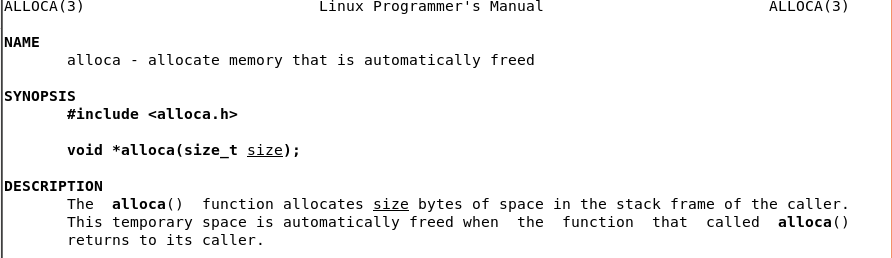
\includegraphics[width=\textwidth]{alloca-man}
\end{frame}

\begin{frame}{writing alloca}
\begin{itemize}
\item how is it possible to write this function???
\item allocating space without overwriting return address???
\end{itemize}
\end{frame}

\begin{frame}[fragile,label=histBSDAlloca]{an historical implementation}
\lstset{
    language=myasm,
    style=smaller,
    moredelim={**[is][\btHL<all:2>]{@2}{2@}},
    moredelim={**[is][\btHL<all:3>]{@3}{3@}},
    moredelim={**[is][\btHL<all:4>]{@4}{4@}},
}
\begin{itemize}
\item 386BSD (1990) 32-bit x86 implementation
\begin{itemize}\item converted to Intel syntax, some comments added\end{itemize}
\end{itemize}
\begin{lstlisting}
alloca:
    pop edx		/*  pop return addr */
    pop @2eax2@		/*  pop amount to allocate */
    mov	ecx, esp
    add	eax, 3		/*  round up to next word */
    and eax, 0xfffffffc
    sub @3esp3@,eax         /* adjust stack pointer for allocation */
    mov	eax,esp 	/* set ret. val. to base of
                               newly allocated space */
    push @4[ecx+8]4@	/* copy possible saved registers */
    push [ecx+4]
    push [ecx+0]
    push @2eax2@		/* dummy to pop at callsite */
    jmp	edx		/* "return" */
\end{lstlisting}
\begin{tikzpicture}[overlay,remember picture]
    \coordinate (placeLow) at ([yshift=2cm]current page.south);
    \coordinate (placeHigh) at ([yshift=5cm]current page.south);
    \tikzset{box/.style={draw=red,very thick,fill=white,anchor=south,align=left}}
    \begin{visibleenv}<2>
        \node[box] at (placeLow) {
            32-bit x86 calling convention: all args on stack
        };
    \end{visibleenv}
    \begin{visibleenv}<3>
        \node[box] at (placeHigh) {
            changing stack pointer \\
            how does caller access local variables on the stack? \\
            assumption: uses a base pointer instead\ldots
        };
    \end{visibleenv}
    \begin{visibleenv}<4>
        \node[box] at (placeHigh) {
            how do they know caller only saves 3 registers? \\
            maybe they wrote the compiler\ldots?
        };
    \end{visibleenv}
\end{tikzpicture}
\end{frame}

\begin{frame}[fragile,label=modernAlloca]{a modern implementation: compiler built-in}
\lstset{
    language=C++,
    style=smaller,
    moredelim={**[is][\btHL<all:2>]{@2}{2@}},
    moredelim={**[is][\btHL<all:3>]{@3}{3@}},
    moredelim={**[is][\btHL<all:4>]{@4}{4@}},
}
\begin{lstlisting}
void foo(int N) {
    char *temp = alloca(N);
    bar(temp);
}
\end{lstlisting}
\lstset{
    language=myasm,
    style=smaller,
    moredelim={**[is][\btHL<all:2>]{@2}{2@}},
    moredelim={**[is][\btHL<all:3>]{@3}{3@}},
    moredelim={**[is][\btHL<all:4>]{@4}{4@}},
}
\begin{lstlisting}
foo: # @foo
  push @2rbp2@
  mov @2rbp, rsp2@
  movsxd rax, edi
  mov rdi, rsp
  add rax, 15
  and rax, -16
  sub rdi, rax
  @3mov rsp, rdi3@
  call bar
  mov @2rsp, rbp2@
  pop @2rbp2@
  ret
\end{lstlisting}
\begin{tikzpicture}[overlay,remember picture]
    \coordinate (placeLow) at ([xshift=3cm,yshift=2cm]current page.south);
    \coordinate (placeHigh) at ([yshift=5cm]current page.south);
    \tikzset{box/.style={draw=red,very thick,fill=white,anchor=south,align=left}}
    \begin{visibleenv}<2>
        \node[box] at (placeLow) {
            use frame pointer --- \\ remember original stack location
        };
    \end{visibleenv}
    \begin{visibleenv}<3>
        \node[box] at (placeLow) {
            rsp becomes rsp - N  \\ (N rounded up to next mult. of 16)
        };
    \end{visibleenv}
\end{tikzpicture}
\end{frame}
